\documentclass[xcolor=dvipsnames,beamer]{beamer} %handout,notes=show

\usepackage{textcomp}
\usepackage[utf8]{inputenc}
% \usepackage{default}
\usepackage{graphicx}
%  \usepackage[pdftex]{hyperref}
\usepackage{url}
\usepackage{amsmath}

% frames have to be fragile
\newif\ifnotes
% \notestrue

%\notestrue


\ifnotes
%\setbeamertemplate{note page}[plain]
\setbeamertemplate{note page}[compress]
\setbeamerfont{note page}{size=\large}
\setbeameroption{show only notes}
%\setbeameroption{show notes}
\usepackage{pgfpages}
\pgfpagesuselayout{2 on 1}[a4paper,border shrink=5mm]%
\else
%\setbeameroption{hide notes}
\fi
%\notesfalse



% nastaveni TypeWriter
%\usepackage{courier}
%\usepackage{lmodern}
%\renewcommand*\ttdefault{txtt}
\DeclareFontShape{OT1}{cmtt}{bx}{n}{<5><6><7><8><9><10><10.95><12><14.4><17.28><20.74><24.88>cmttb10}{}


% \usepackage{verbatim}
\usepackage[absolute,overlay]{textpos}

\usepackage{listings}
% \usepackage{courier}
\definecolor{grey}{RGB}{70,70,70}
\definecolor{green}{RGB}{0,255,0}
\definecolor{red}{RGB}{202,53,53}
\definecolor{lightGrey}{RGB}{250,250,250}
\definecolor{darkGrey}{RGB}{50,50,50}


\usepackage{color}
\definecolor{lightgray}{rgb}{.9,.9,.9}
\definecolor{darkgray}{rgb}{.4,.4,.4}
\definecolor{purple}{rgb}{0.65, 0.12, 0.82}

% \usetheme{Boadilla}
\usetheme{Goettingen}
% \usetheme{Montpellier}
% \usetheme{Warsaw}
% \usetheme{Madrid}
% \usetheme{Szeged}
% \useoutertheme{infolines}
% \usecolortheme[named=MidnightBlue]{structure}
\usecolortheme[named=PineGreen]{structure}
% \setbeamertemplate{navigation symbols}{}




\title[FOSS4G - OSHW]
{Combining FOSS4G \& Open Hardware\\
for\\ Research \& Monitoring in Southern Asia}
%\subtitle{SVO\v{C}}
%\pdforstring{}{}
\author[Yann Chemin]
{\vspace{40pt}\\
Yann Chemin}

\institute[IWMI - U of Moratuwa]
{International Water Management Institute\\
 \vspace{5pt}
University of Moratuwa, Faculty of Architecture
\begin{center}
 
\includegraphics[width=4cm]{foss4g2013logo_s}
\end{center}
}
\date{\tiny November 5th, 2013}


%\AtBeginSection[]{\begin{frame}\frametitle{Obsah}%
%\tableofcontents[currentsection ]\end{frame}}
%\AtBeginSubsection[]
%{
%  \begin{frame}<beamer>
%  \frametitle{Obsah}
%  \tableofcontents[currentsection,currentsubsection]
%  \end{frame}
%}

\setbeamercovered{transparent}

\hypersetup{%
	pdfauthor={Yann Chemin},%
	pdfsubject={Presentation},%
    pdfkeywords={FOSS4G, OSHW, RaspberryPI, ET, Raingauge, Road Condition, OSGEO}
}

\usepackage{listings}
\lstdefinestyle{C++}{%
  % language
  language=C++, % [ANSI]C++, GNU, ISO, Visual
  basicstyle=\ttfamily\small,
  commentstyle=\itshape,
  keywordstyle=\bfseries, % needs another \ttdefault
  showstringspaces=false,
  stringstyle=,
  identifierstyle=,
  % working with latex
  escapeinside={//lst}{\^^M}  
}

\lstset{%
%  frame=trBL,
%  backgroundcolor=\color{},
  linewidth=\textwidth,
  % working with latex
  gobble=2,
  % float
  nolol=false,
  numberbychapter=true,
  captionpos=t,% tb
  % breaking lines
  breaklines=true,
  breakatwhitespace=true,
  breakindent=10em,
  breakautoindent=true,
  prebreak={},
  postbreak={},
  %document default style
    basicstyle=\ttfamily
}


%\lstlistlistingname % The header name for the list of listings.
%\lstlistingname % The caption label for listings.

\lstnewenvironment{cmdline}[1][]
{\lstset{
  style=C++,
  #1}}
{}

\lstnewenvironment{scpp}[1][]
{\lstset{
  style=C++,
  #1}}
{}

\lstnewenvironment{ncpp}[1][]
{\lstset{
  style=C++,
  numbers=left, 
  numberstyle=\scriptsize, 
  stepnumber=1,
  numbersep=5pt,
  #1}}
{}

\lstnewenvironment{fcpp}[1][]
{\lstset{
  style=C++,
  float,
   % line numbers
  numbers=left, 
  numberstyle=\scriptsize, 
  stepnumber=1,
  numbersep=5pt,
  #1}}
{}


\lstnewenvironment{lcpp}[1][]
{\lstset{%
style=C++,
numbers=left, 
numberstyle=\scriptsize, 
stepnumber=1,
numbersep=5pt,
xleftmargin=12pt,
breakautoindent=false,
breaklines=false,%
#1}}{}

\lstnewenvironment{smallcpp}[1][]
{\lstset{%
style=C++,
numbers=left, 
numberstyle=\tiny, 
stepnumber=1,
numbersep=5pt,
xleftmargin=12pt,
breakautoindent=false,
breaklines=false,%
basicstyle=\ttfamily\scriptsize,
#1}}{}


\lstnewenvironment{pscpp}[1][]
{\lstset{%
style=C++,
xleftmargin=12pt,
breakautoindent=false,
breaklines=false,
#1}}{}


%\lstset{index={square},index={[2]root}}


\newcommand{\overovaciref}[1]{{\scriptsize(\ref{#1})}}


\usepackage{tipa}
\newcommand{\pron}[2]{#1 [#2]}

%%%%%%%%%%%%%%%%%%%%%%%%%%%%%%%%%%%%%%%%%%%%%%%%%%%%%%%%%%%%%%%%%%%%
% TOC frame setup
%%%%%%%%%%%%%%%%%%%%%%%%%%%%%%%%%%%%%%%%%%%%%%%%%%%%%%%%%%%%%%%%%%%%
\usepackage{multicol}
\colorlet{mycolor}{orange!80!black}% change this color to suit your needs
\AtBeginSection[]{
  \setbeamercolor{section in toc shaded}{use=structure,fg=structure.fg}
  \setbeamercolor{section in toc}{fg=mycolor}
  \setbeamercolor{subsection in toc shaded}{fg=black}
  \setbeamercolor{subsection in toc}{fg=mycolor}
  \frame<beamer>{\begin{multicols}{2}
  \frametitle{Outline}
  \setcounter{tocdepth}{2}  
  \tableofcontents[currentsection,subsections]
\end{multicols} 
 }
}

\setbeamercolor{author in head/foot}{fg=white}
\setbeamercolor{title in head/foot}{fg=white}
\setbeamercolor{section in head/foot}{fg=mycolor}
\setbeamertemplate{section in head/foot shaded}{\color{white!70!black}\insertsectionhead}
\setbeamercolor{subsection in head/foot}{fg=mycolor}
\setbeamertemplate{subsection in head/foot shaded}{\color{white!70!black}\insertsubsectionhead}
\setbeamercolor{frametitle}{fg=white}
\setbeamercolor{framesubtitle}{fg=white}

%%%%%%%%%%%%%%%%%%%%%%%%%%%%%%%%%%%%%%%%%%%%%%%%%%%%%%%%%%%%%%%%%%%%
%%%%%%%%%%%%%%%%%%%%%%%%%%%%%%%%%%%%%%%%%%%%%%%%%%%%%%%%%%%%%%%%%%%%
%%%%%%%%%%%%%%%%%%%%%%%%%%%%%%%%%%%%%%%%%%%%%%%%%%%%%%%%%%%%%%%%%%%%
\begin{document}


%%%%%%%%%%%%%%%%%%%%%%%%%%%%%%%%%%%%%%%%%%%%%%%%%%%%%%%%%%%%%%%%%%%%
\begin{frame}
 \maketitle
\end{frame}
%%%%%%%%%%%%%%%%%%%%%%%%%%%%%%%%%%%%%%%%%%%%%%%%%%%%%%%%%%%%%%%%%%%%

%%%%%%%%%%%%%%%%%%%%%%%%%%%%%%%%%%%%%%%%%%%%%%%%%%%%%%%%%%%%%%%%%%%%
\begin{frame}{Contents}
 \begin{multicols}{2}
  \setcounter{tocdepth}{2}  
  \tableofcontents
 \end{multicols} 
\end{frame}
%%%%%%%%%%%%%%%%%%%%%%%%%%%%%%%%%%%%%%%%%%%%%%%%%%%%%%%%%%%%%%%%%%%%

%%%%%%%%%%%%%%%%%%%%%%%%%%%%%%%%%%%%%%%%%%%%%%%%%%%%%%%%%%%%%%%%%%%%
\begin{frame}[fragile]{CGIAR}

Consultative Group for International Agricultural Research\\
Ratified on October 2nd, 2013\\
Full Open Access \& Open Source\\
Research data and publication

\begin{columns}[l]
\column{0.5\textwidth}
\begin{center}
\begin{itemize}
 \item International Public Goods
 \item Public Domain
 \item Publications Open Access
 \item FOSS models and algorithms
\end{itemize}
\end{center}

\column{0.5\textwidth}
\begin{center}
  
\includegraphics[width=1.5cm]{CGIAR_Green}
  \hspace{5mm}
  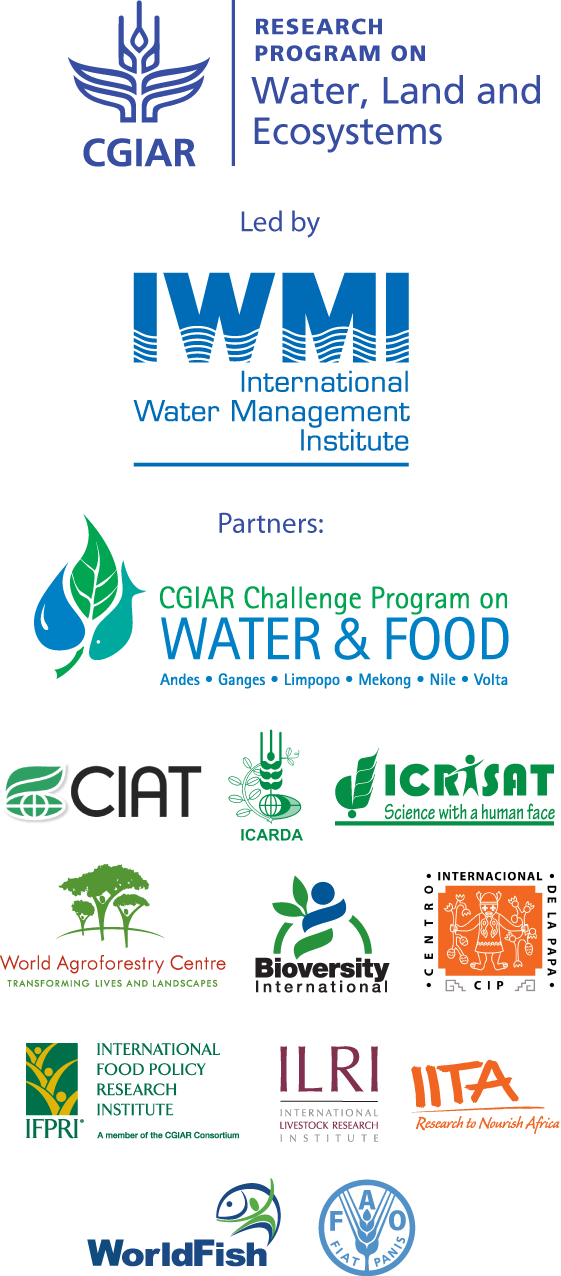
\includegraphics[width=2cm]{WLE_and_partners-vertical_logo_strip.png}
\end{center}
\end{columns}
\vspace{5mm} 2018: all 15 CG centres, already FOSS4G Lab:
(\href{http://gsl.worldagroforestry.org}{gsl.worldagroforestry.org})
\end{frame}


\section{Introduction}
%%%%%%%%%%%%%%%%%%%%%%%%%%%%%%%%%%%%%%%%%%%%%%%%%%%%%%%%%%%%%%%%%%%%
\begin{frame}[fragile]{Overview}

FOSS4G and Open Hardware\\
Developed together in new avenues
\newline\linebreak

\begin{itemize}
 \item Evapotranspiration calibration \& modeling
%  \item Rainwater harvesting monitoring
 \item Road condition monitoring
 \item Rural tanks evaporation modeling
\end{itemize}
\end{frame}

\section{PyWPS+MWS}
\subsection{Rationale}
%%%%%%%%%%%%%%%%%%%%%%%%%%%%%%%%%%%%%%%%%%%%%%%%%%%%%%%%%%%%%%%%%%%%
\begin{frame}[fragile]{Rationale}

\begin{center}
  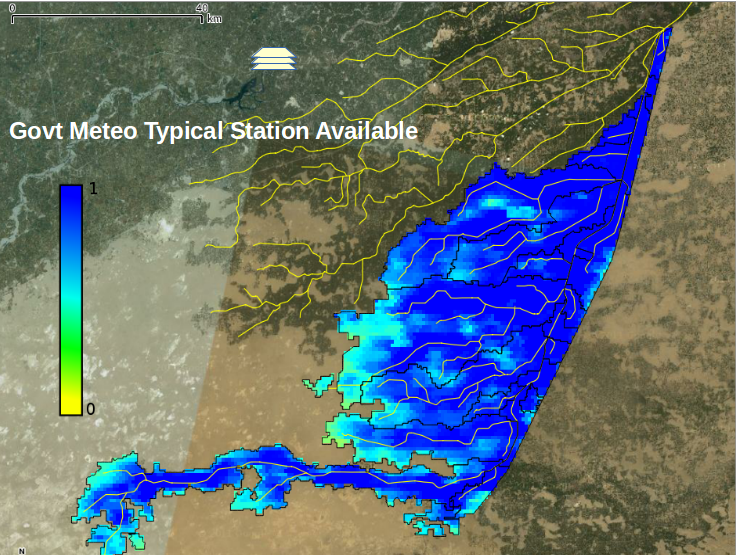
\includegraphics[width=10cm]{MWS_v1_deltaT_rationale_0}
\end{center}

\end{frame}

%%%%%%%%%%%%%%%%%%%%%%%%%%%%%%%%%%%%%%%%%%%%%%%%%%%%%%%%%%%%%%%%%%%%
\begin{frame}[fragile]{Rationale}

\begin{center}
  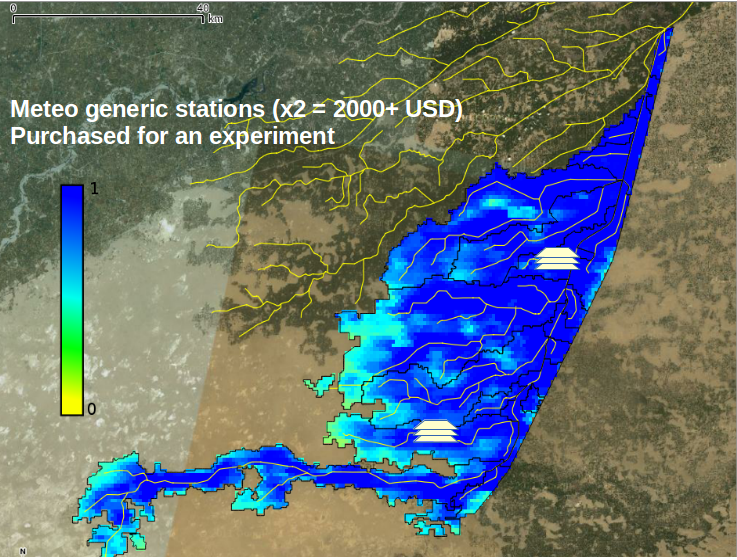
\includegraphics[width=10cm]{MWS_v1_deltaT_rationale_1}
\end{center}

\end{frame}

%%%%%%%%%%%%%%%%%%%%%%%%%%%%%%%%%%%%%%%%%%%%%%%%%%%%%%%%%%%%%%%%%%%%
\begin{frame}[fragile]{Rationale}

\begin{center}
  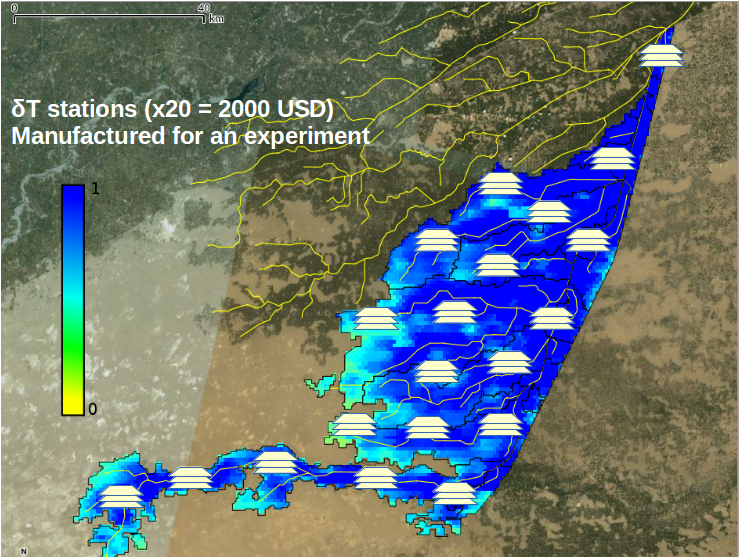
\includegraphics[width=10cm]{MWS_v1_deltaT_rationale_2}
\end{center}

\end{frame}

\subsection{MWS}
%%%%%%%%%%%%%%%%%%%%%%%%%%%%%%%%%%%%%%%%%%%%%%%%%%%%%%%%%%%%%%%%%%%%
\begin{frame}[fragile]{Open Source Hardware Micro Weather Station v1}

Micro Weather Station v1:\\
Temperature Profiler for ET models calibration
\vspace{5mm}
\begin{itemize}
 \item Arduino Pro 3.3V
 \item Water-proof Digital Temperature Sensors
 \item Li-ion Battery + Solar Panel
 \item OpenLog data logger with SD card
 \item Cost $<$ 100 USD
\end{itemize}
\begin{flushright}
  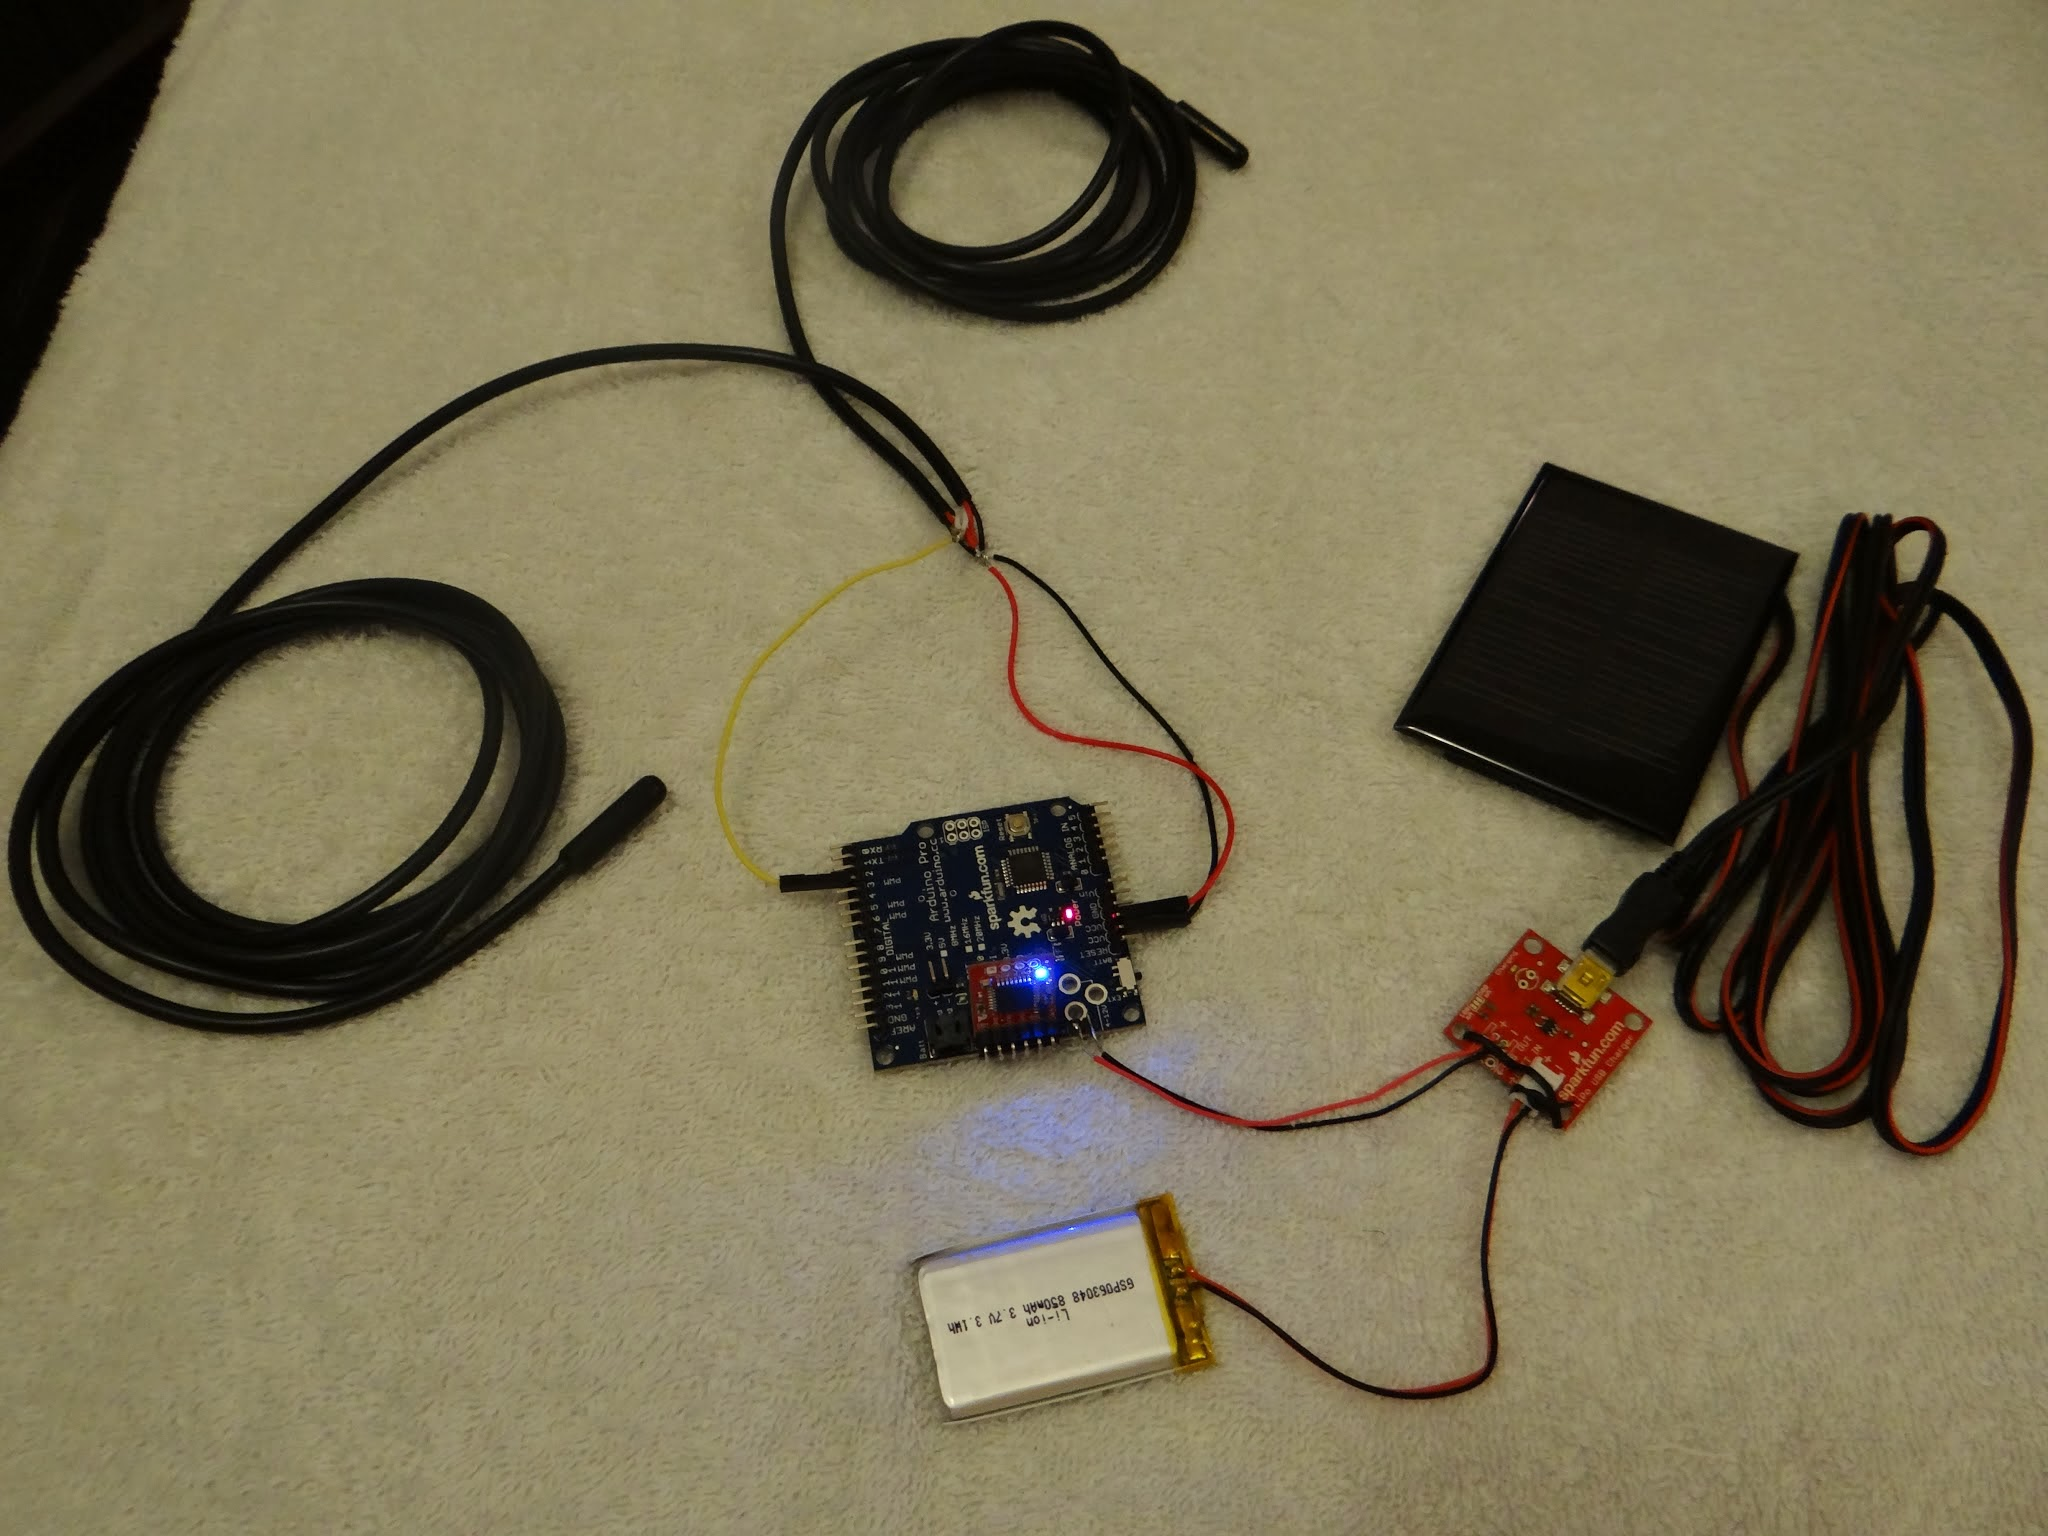
\includegraphics[width=5cm]{MWS}
  \hspace{5mm}
  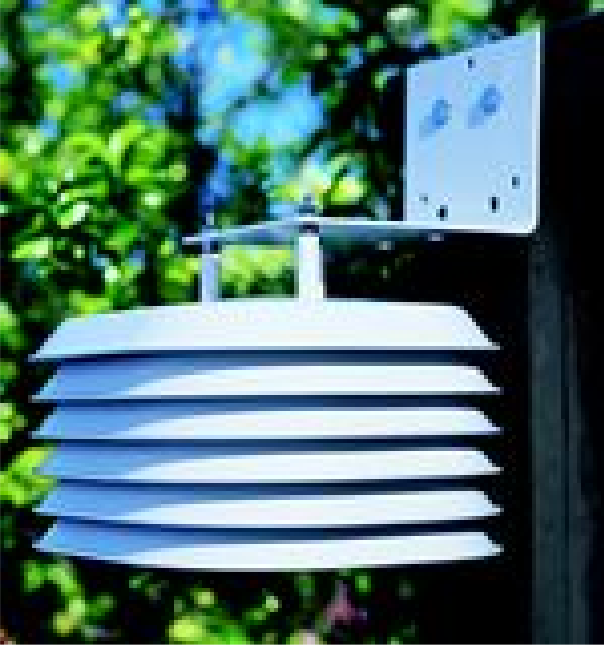
\includegraphics[width=2cm]{MWS_radshield}
\end{flushright}
\end{frame}

\subsection{MWS parts}
%%%%%%%%%%%%%%%%%%%%%%%%%%%%%%%%%%%%%%%%%%%%%%%%%%%%%%%%%%%%%%%%%%%%
\begin{frame}[fragile]{Open Source Hardware Micro Weather Station v1}

\begin{center}
OpenLog + Arduino Pro\\
\vspace{5mm}
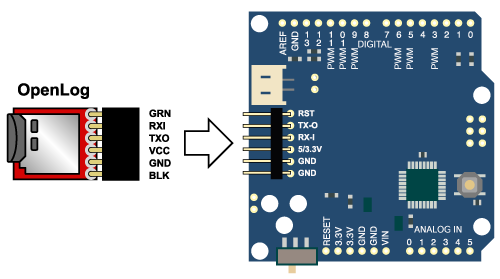
\includegraphics[width=5cm]{Arduino_OpenLog}
\end{center}

\begin{flushright}
  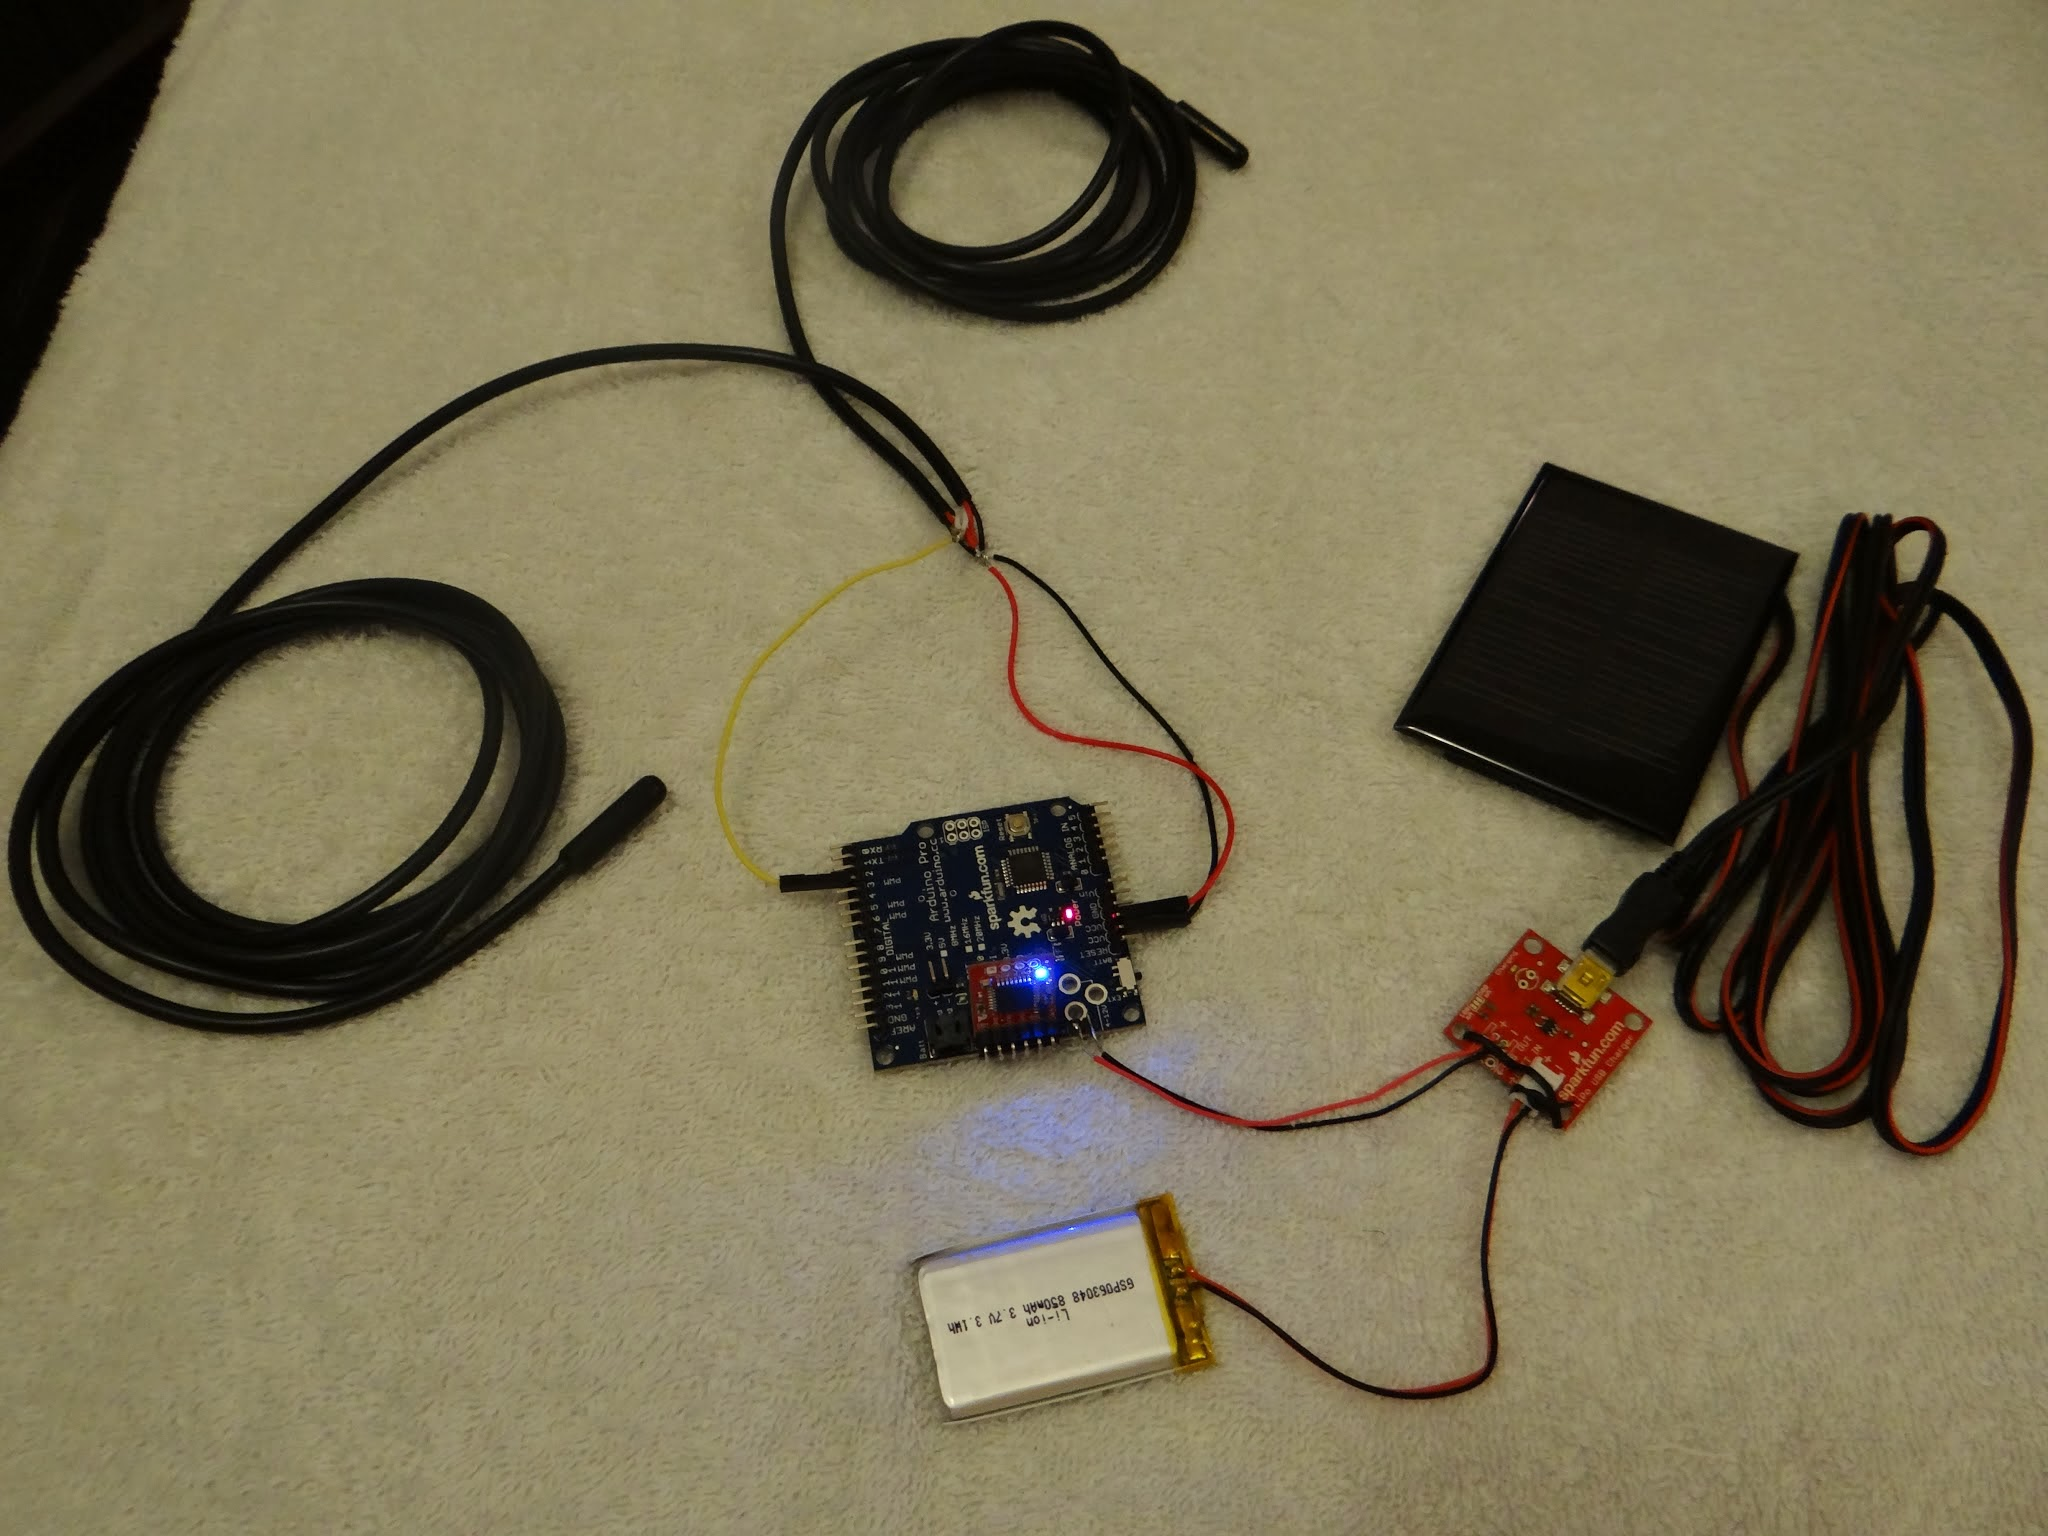
\includegraphics[width=5cm]{MWS}
  \hspace{5mm}
  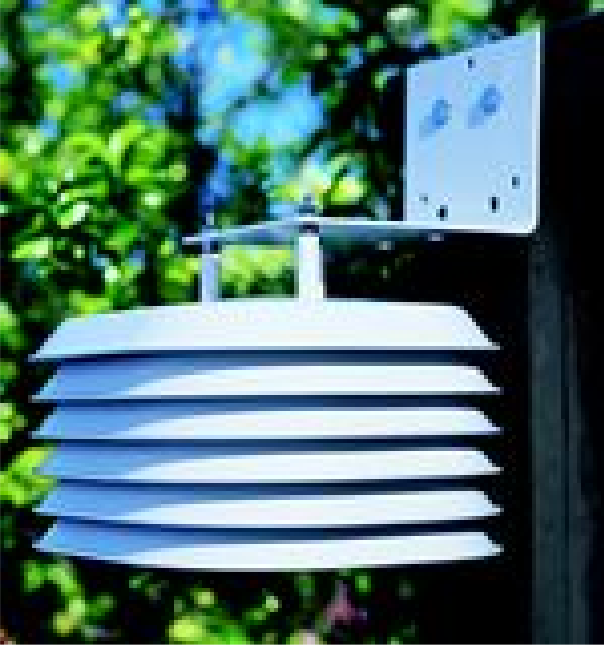
\includegraphics[width=2cm]{MWS_radshield}
\end{flushright}
\end{frame}

\subsection{MWS Setup}
%%%%%%%%%%%%%%%%%%%%%%%%%%%%%%%%%%%%%%%%%%%%%%%%%%%%%%%%%%%%%%%%%%%%
\begin{frame}[fragile]{MWS Setup}

\begin{center}
 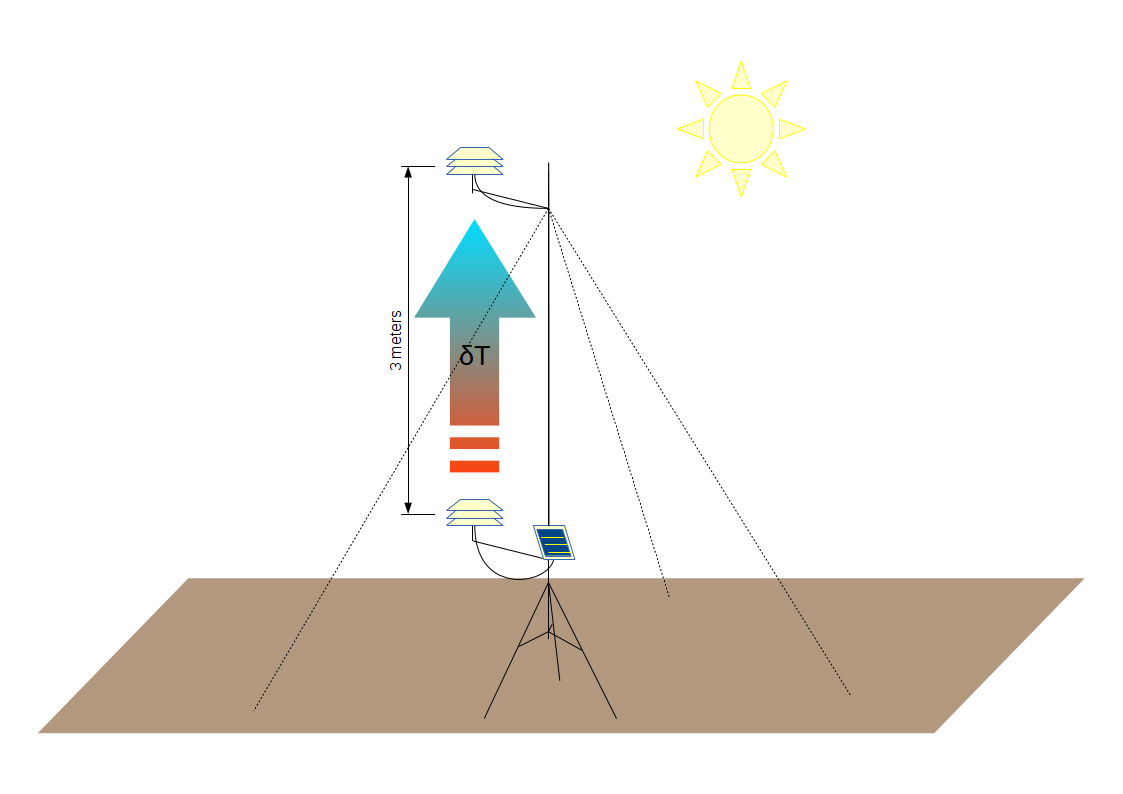
\includegraphics[width=10cm]{MWS_v1_deltaT_sketch_hot}
\end{center}

\end{frame}

%%%%%%%%%%%%%%%%%%%%%%%%%%%%%%%%%%%%%%%%%%%%%%%%%%%%%%%%%%%%%%%%%%%%
\begin{frame}[fragile]{MWS Setup}

\begin{center}
 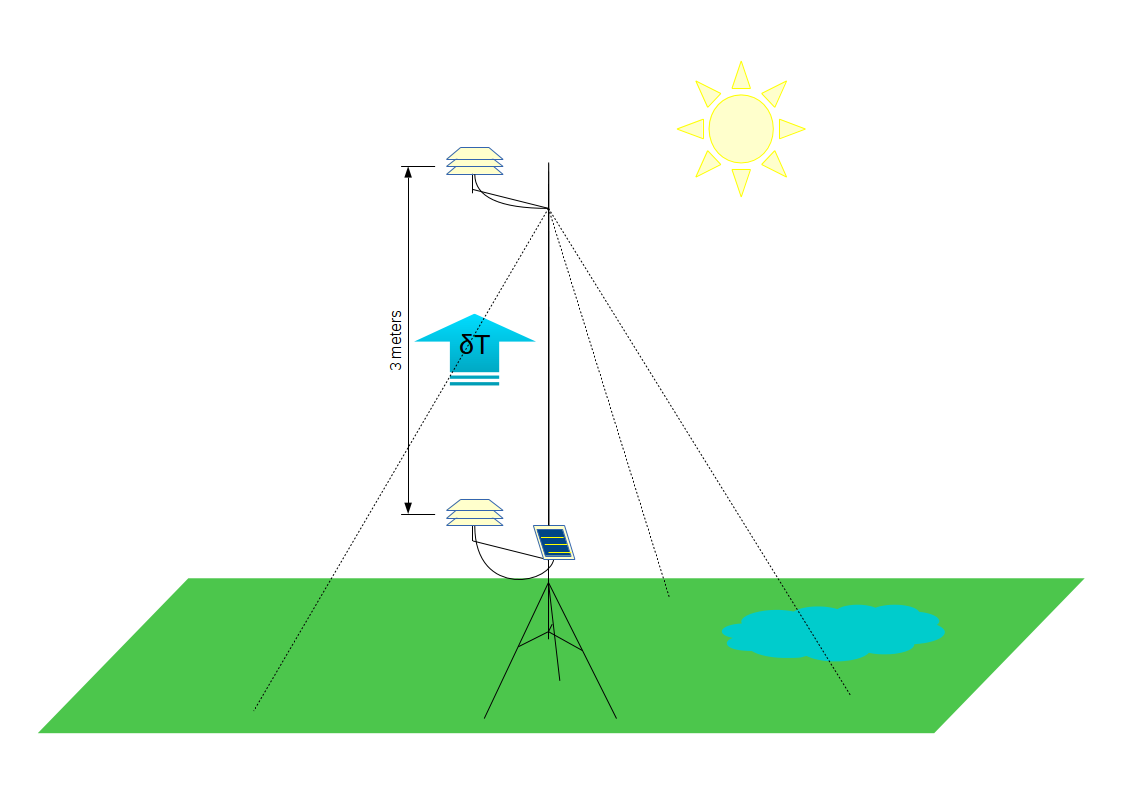
\includegraphics[width=10cm]{MWS_v1_deltaT_sketch_cold}
\end{center}

\end{frame}

\subsection{GRASS GIS}
%%%%%%%%%%%%%%%%%%%%%%%%%%%%%%%%%%%%%%%%%%%%%%%%%%%%%%%%%%%%%%%%%%%%
\begin{frame}[fragile]{GRASS GIS framework}

\begin{center}
 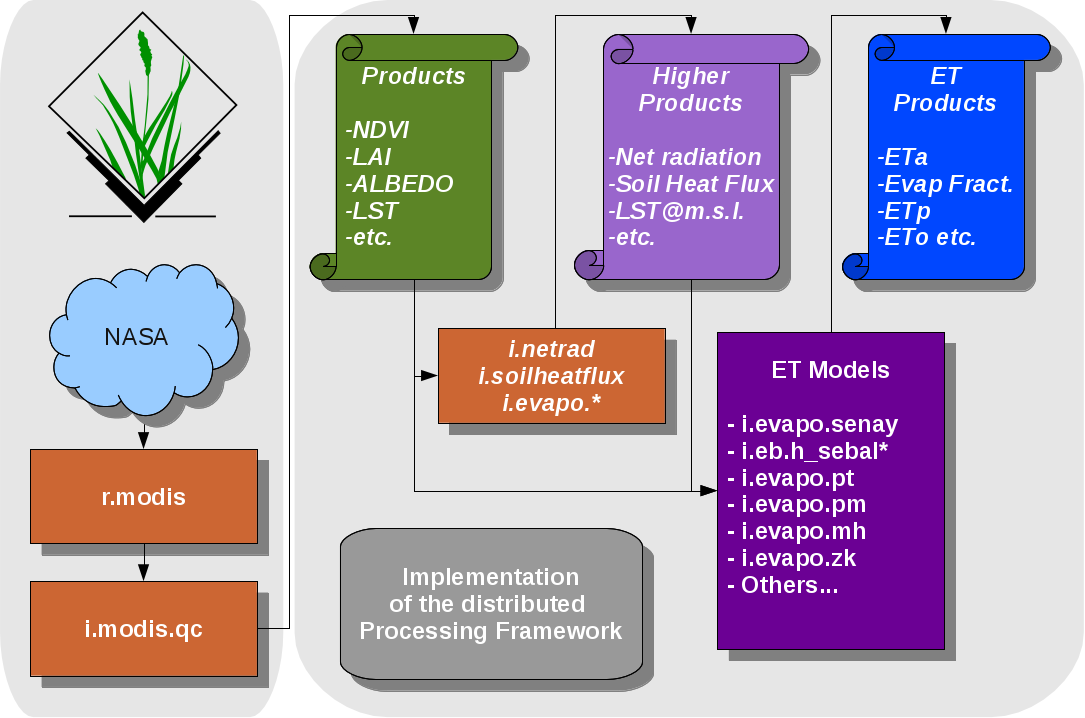
\includegraphics[width=8.5cm]{architecture_implementation}
\end{center}

\end{frame}

\subsection{metaModule}
%%%%%%%%%%%%%%%%%%%%%%%%%%%%%%%%%%%%%%%%%%%%%%%%%%%%%%%%%%%%%%%%%%%%
\begin{frame}[fragile]{metaModule Concept}

Pythonizing GRASS:\\ From Shell commands to Python functions 

\begin{block}{metaModule concept}
\begin{enumerate}
 \item {\bf GRASS GIS:} Specific image processing modules
 \item {\bf PyWPS:} G modules called by Python
 \item {\bf GRASS script:} G mod. called by Python: metaModule
 \item {\bf pyGRASS:} G mod. called as Python fun.: metaModule
 \item {\bf PyWPS v4:} pyGRASS metaModule used directly \textcolor{orange}{\bf{(TODO)}}
\end{enumerate}

\end{block}

\end{frame}

\subsection{pyGRASS}
%%%%%%%%%%%%%%%%%%%%%%%%%%%%%%%%%%%%%%%%%%%%%%%%%%%%%%%%%%%%%%%%%%%%
\begin{frame}[fragile]{pyGRASS metaModule}

\begin{center}
 Summary for Landsat pyGRASS metaModule
 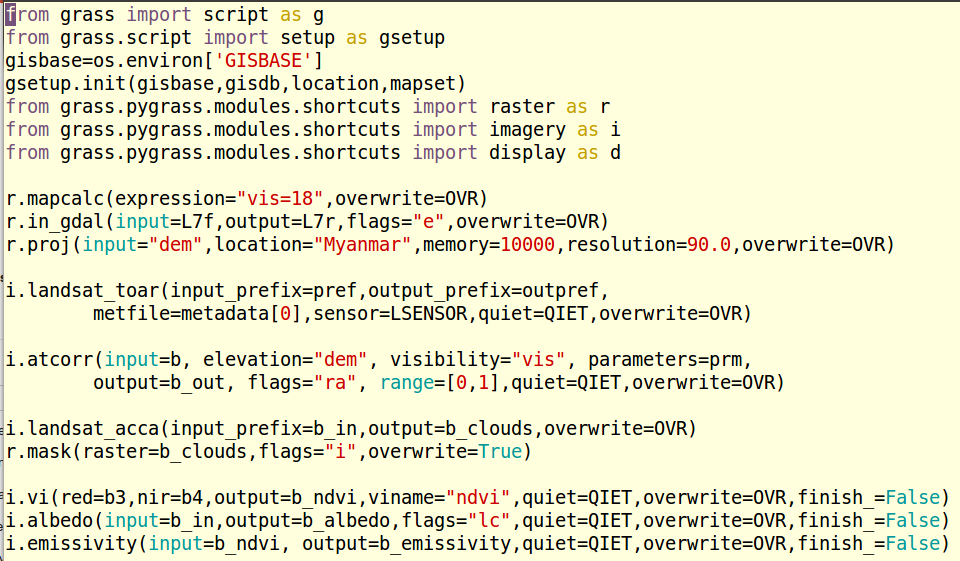
\includegraphics[width=10cm]{pyGRASS1}\\
 \href{http://grasswiki.osgeo.org/wiki/Python/pygrass}{http://grasswiki.osgeo.org/wiki/Python/pygrass}
\end{center}

\end{frame}

%%%%%%%%%%%%%%%%%%%%%%%%%%%%%%%%%%%%%%%%%%%%%%%%%%%%%%%%%%%%%%%%%%%%
\begin{frame}[fragile]{Equity of water use in irrigation systems}

Irrigation water monitoring \& management
\begin{itemize}
 \item Map: Uniform colour is equity of water distribution
 \item Graph: Irrigation system equity (mm/d, daily, 12 years)
\end{itemize}

\begin{columns}[l]
\column{0.4\textwidth}
\begin{center}
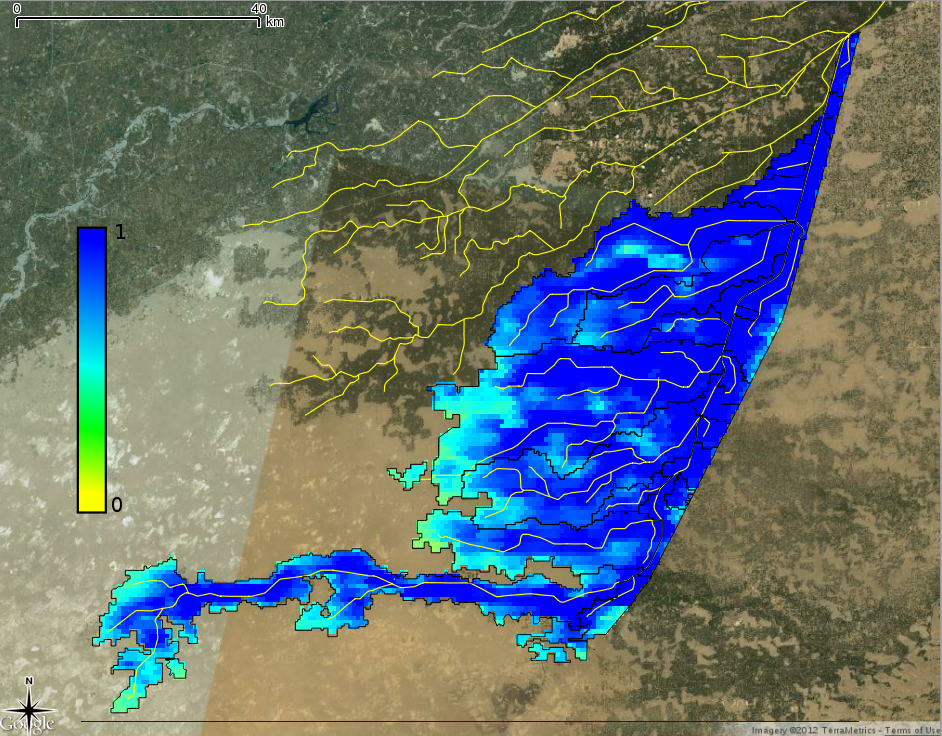
\includegraphics[width=4cm]{fess2012ef}
\end{center}

\column{0.6\textwidth}
\begin{flushleft}
  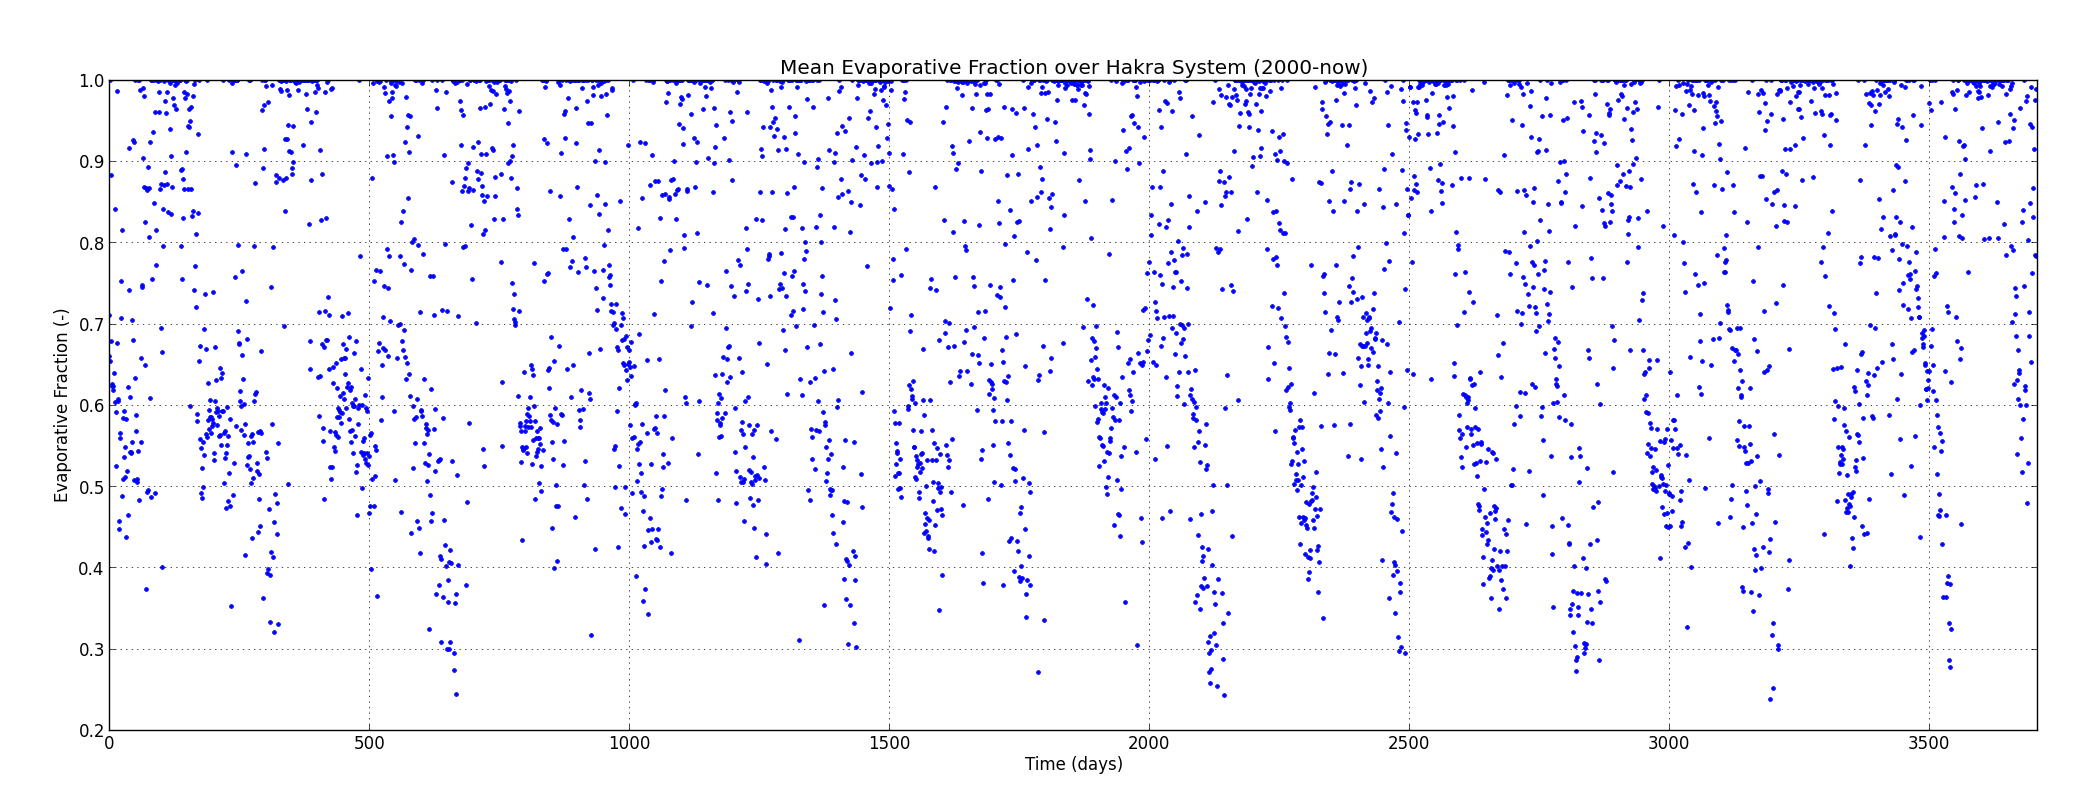
\includegraphics[width=8cm]{fess2012meaneftemporal}
\end{flushleft}
\end{columns}
% Evaporative Fraction 2012 October 4th Hakra, Punjab, Pakistan ~4000 images (2000-2012)
\end{frame}

\subsection{PyWPS}
%%%%%%%%%%%%%%%%%%%%%%%%%%%%%%%%%%%%%%%%%%%%%%%%%%%%%%%%%%%%%%%%%%%%
\begin{frame}[fragile]{PyWPS}
 Developed by Jachym Cepicky (\href{http://les-ejk.cz/}{http://les-ejk.cz/})
\begin{columns}[l]
\column{0.7\textwidth}
 \begin{itemize}
  \item OGC WPS standard
  \item Server side
  \item Written in Python Language
  \item Version 4 in the making
  \item v4 Low-level API: integration with GRASS GIS
  \item v4 Possible pyGRASS support
 \end{itemize}

\column{0.3\textwidth}
\begin{flushright}
  
\includegraphics[width=4cm]{pywps}
\end{flushright}
\end{columns}
\hspace{10mm}
% {\small {\bf from} pywps {\bf import} (Process, Service, WPSResponse, LiteralInput,
%                    ComplexInput, Format, FileReference)}
\end{frame}

%%%%%%%%%%%%%%%%%%%%%%%%%%%%%%%%%%%%%%%%%%%%%%%%%%%%%%%%%%%%%%%%%%%%
\begin{frame}[fragile]{PyWPS system used in FESS study}

\begin{block}{PyWPS v2 style}
\begin{center}
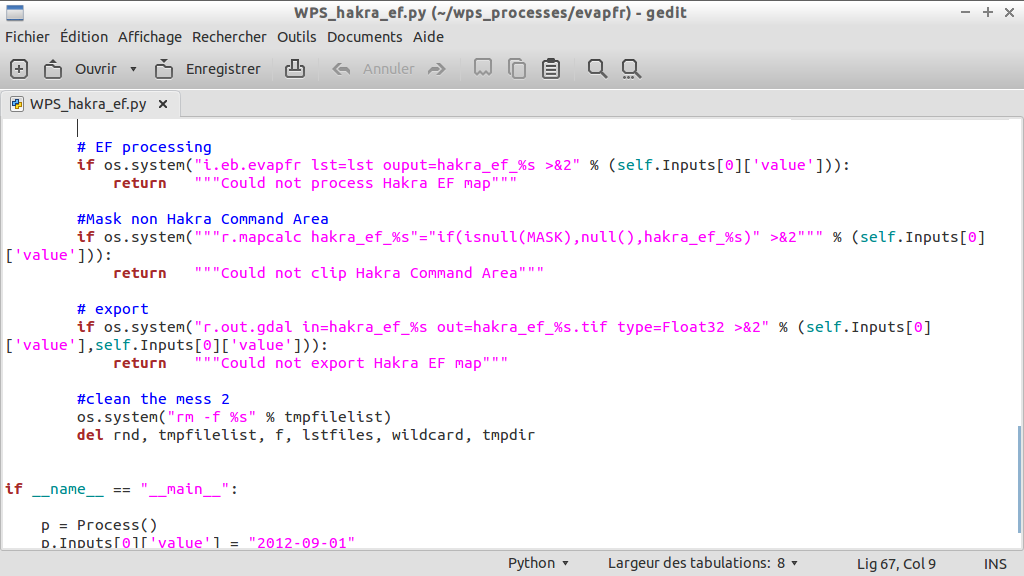
\includegraphics[width=10cm]{pywps_hakra}
\end{center}
\end{block}
\end{frame}

\section{Road condition}
\subsection{Rationale}
%%%%%%%%%%%%%%%%%%%%%%%%%%%%%%%%%%%%%%%%%%%%%%%%%%%%%%%%%%%%%%%%%%%%
\begin{frame}[fragile]{Road Condition Monitoring}

University of Moratuwa, F. of Archit., Urban Planning\\
\vspace{5mm}
\begin{itemize}
 \item {\bf Road condition:} chronic issue in Sri Lanka
 \item {\bf RDA:} few IMU Vehicles (V. Expensive)
 \item {\bf Challenge:} OSHW+FOSS4G $<$ 100 USD/vehicle 
 \item {\bf Solution:} GDAL/OGR + RaspberryPI
\end{itemize}
\vspace{5mm}
\begin{flushleft}
 
\includegraphics[height=2.5cm]{uoMoratuwa}
 \hspace{5mm}
 
\includegraphics[height=2.5cm]{uoMoratuwa_foa}
 \hspace{15mm}
\end{flushleft}
\end{frame}

\subsection{Components}
%%%%%%%%%%%%%%%%%%%%%%%%%%%%%%%%%%%%%%%%%%%%%%%%%%%%%%%%%%%%%%%%%%%%
\begin{frame}[fragile]{Road Condition Monitoring}

System setup on a vehicle:
\vspace{5mm}
\begin{itemize}
 \item RaspberryPI
 \item + XloBorg Accelerometer
 \item + GPS 
 \item + Python-OGR
\end{itemize}

\begin{center}
 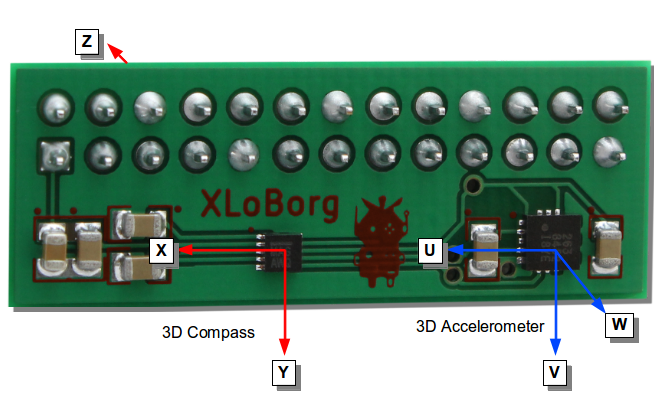
\includegraphics[width=5cm]{xloborg_axis_details}
\end{center}
\end{frame}

\subsection{System}
%%%%%%%%%%%%%%%%%%%%%%%%%%%%%%%%%%%%%%%%%%%%%%%%%%%%%%%%%%%%%%%%%%%%
\begin{frame}[fragile]{Road Condition Monitoring}

Python-OGR reporting Z-axis anomalies into road Shapefiles\\
by integrating Xloborg and GPS data

\begin{center}
 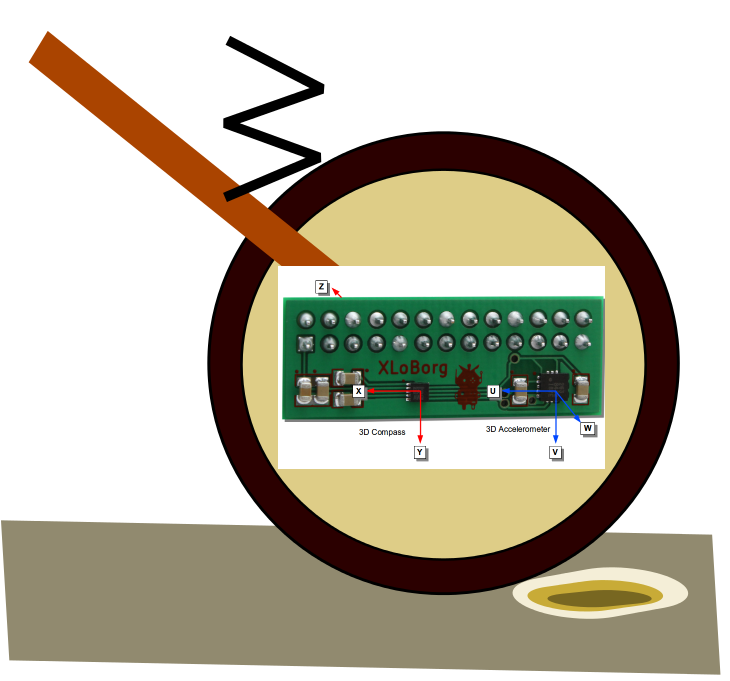
\includegraphics[width=6cm]{road_condition}
 \hspace{5mm}
 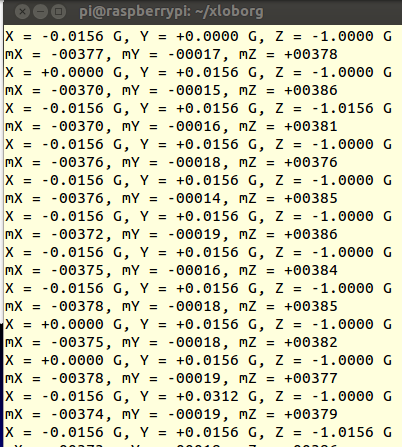
\includegraphics[width=2cm]{accelerometer_data}
\end{center}

\end{frame}

\section{Small Tanks Monitoring}
\subsection{Rationale}
%%%%%%%%%%%%%%%%%%%%%%%%%%%%%%%%%%%%%%%%%%%%%%%%%%%%%%%%%%%%%%%%%%%%
\begin{frame}[fragile]{Rationale}

Water Resources Monitoring in Sri Lanka\\
Trans-basin water, Jaffna city pipeline, etc.
\vspace{5mm}
\begin{block}{Characteristics}
\begin{itemize}
 \item Rural tanks (several thousands!)
 \item Cascade systems (interconnected)
 \item Water Storage capacity changes regularly
 \item Evaporative losses less known
\end{itemize}
\vspace{5mm}
Calibration of evaporative losses\\
and regular monitoring are much needed

\end{block}
\end{frame}

\subsection{Autoboat}
%%%%%%%%%%%%%%%%%%%%%%%%%%%%%%%%%%%%%%%%%%%%%%%%%%%%%%%%%%%%%%%%%%%%
\begin{frame}[fragile]{{\bf Amitomi} Autonomous Survey Boat}

{\bf Amitomi} is a 1m-class autonomous sailing boat\\
Designed to survey small tanks temperature gradient\\
for calibrating Evaporation models\\
\vspace{5mm}
{\it \href{https://sites.google.com/site/amitomiautoboat}
{https://sites.google.com/site/amitomiautoboat}}
\begin{columns}[l]
\column[t]{0.5\textwidth}
\begin{center}
 RaspberryPI as AmiTomi\newline\linebreak
 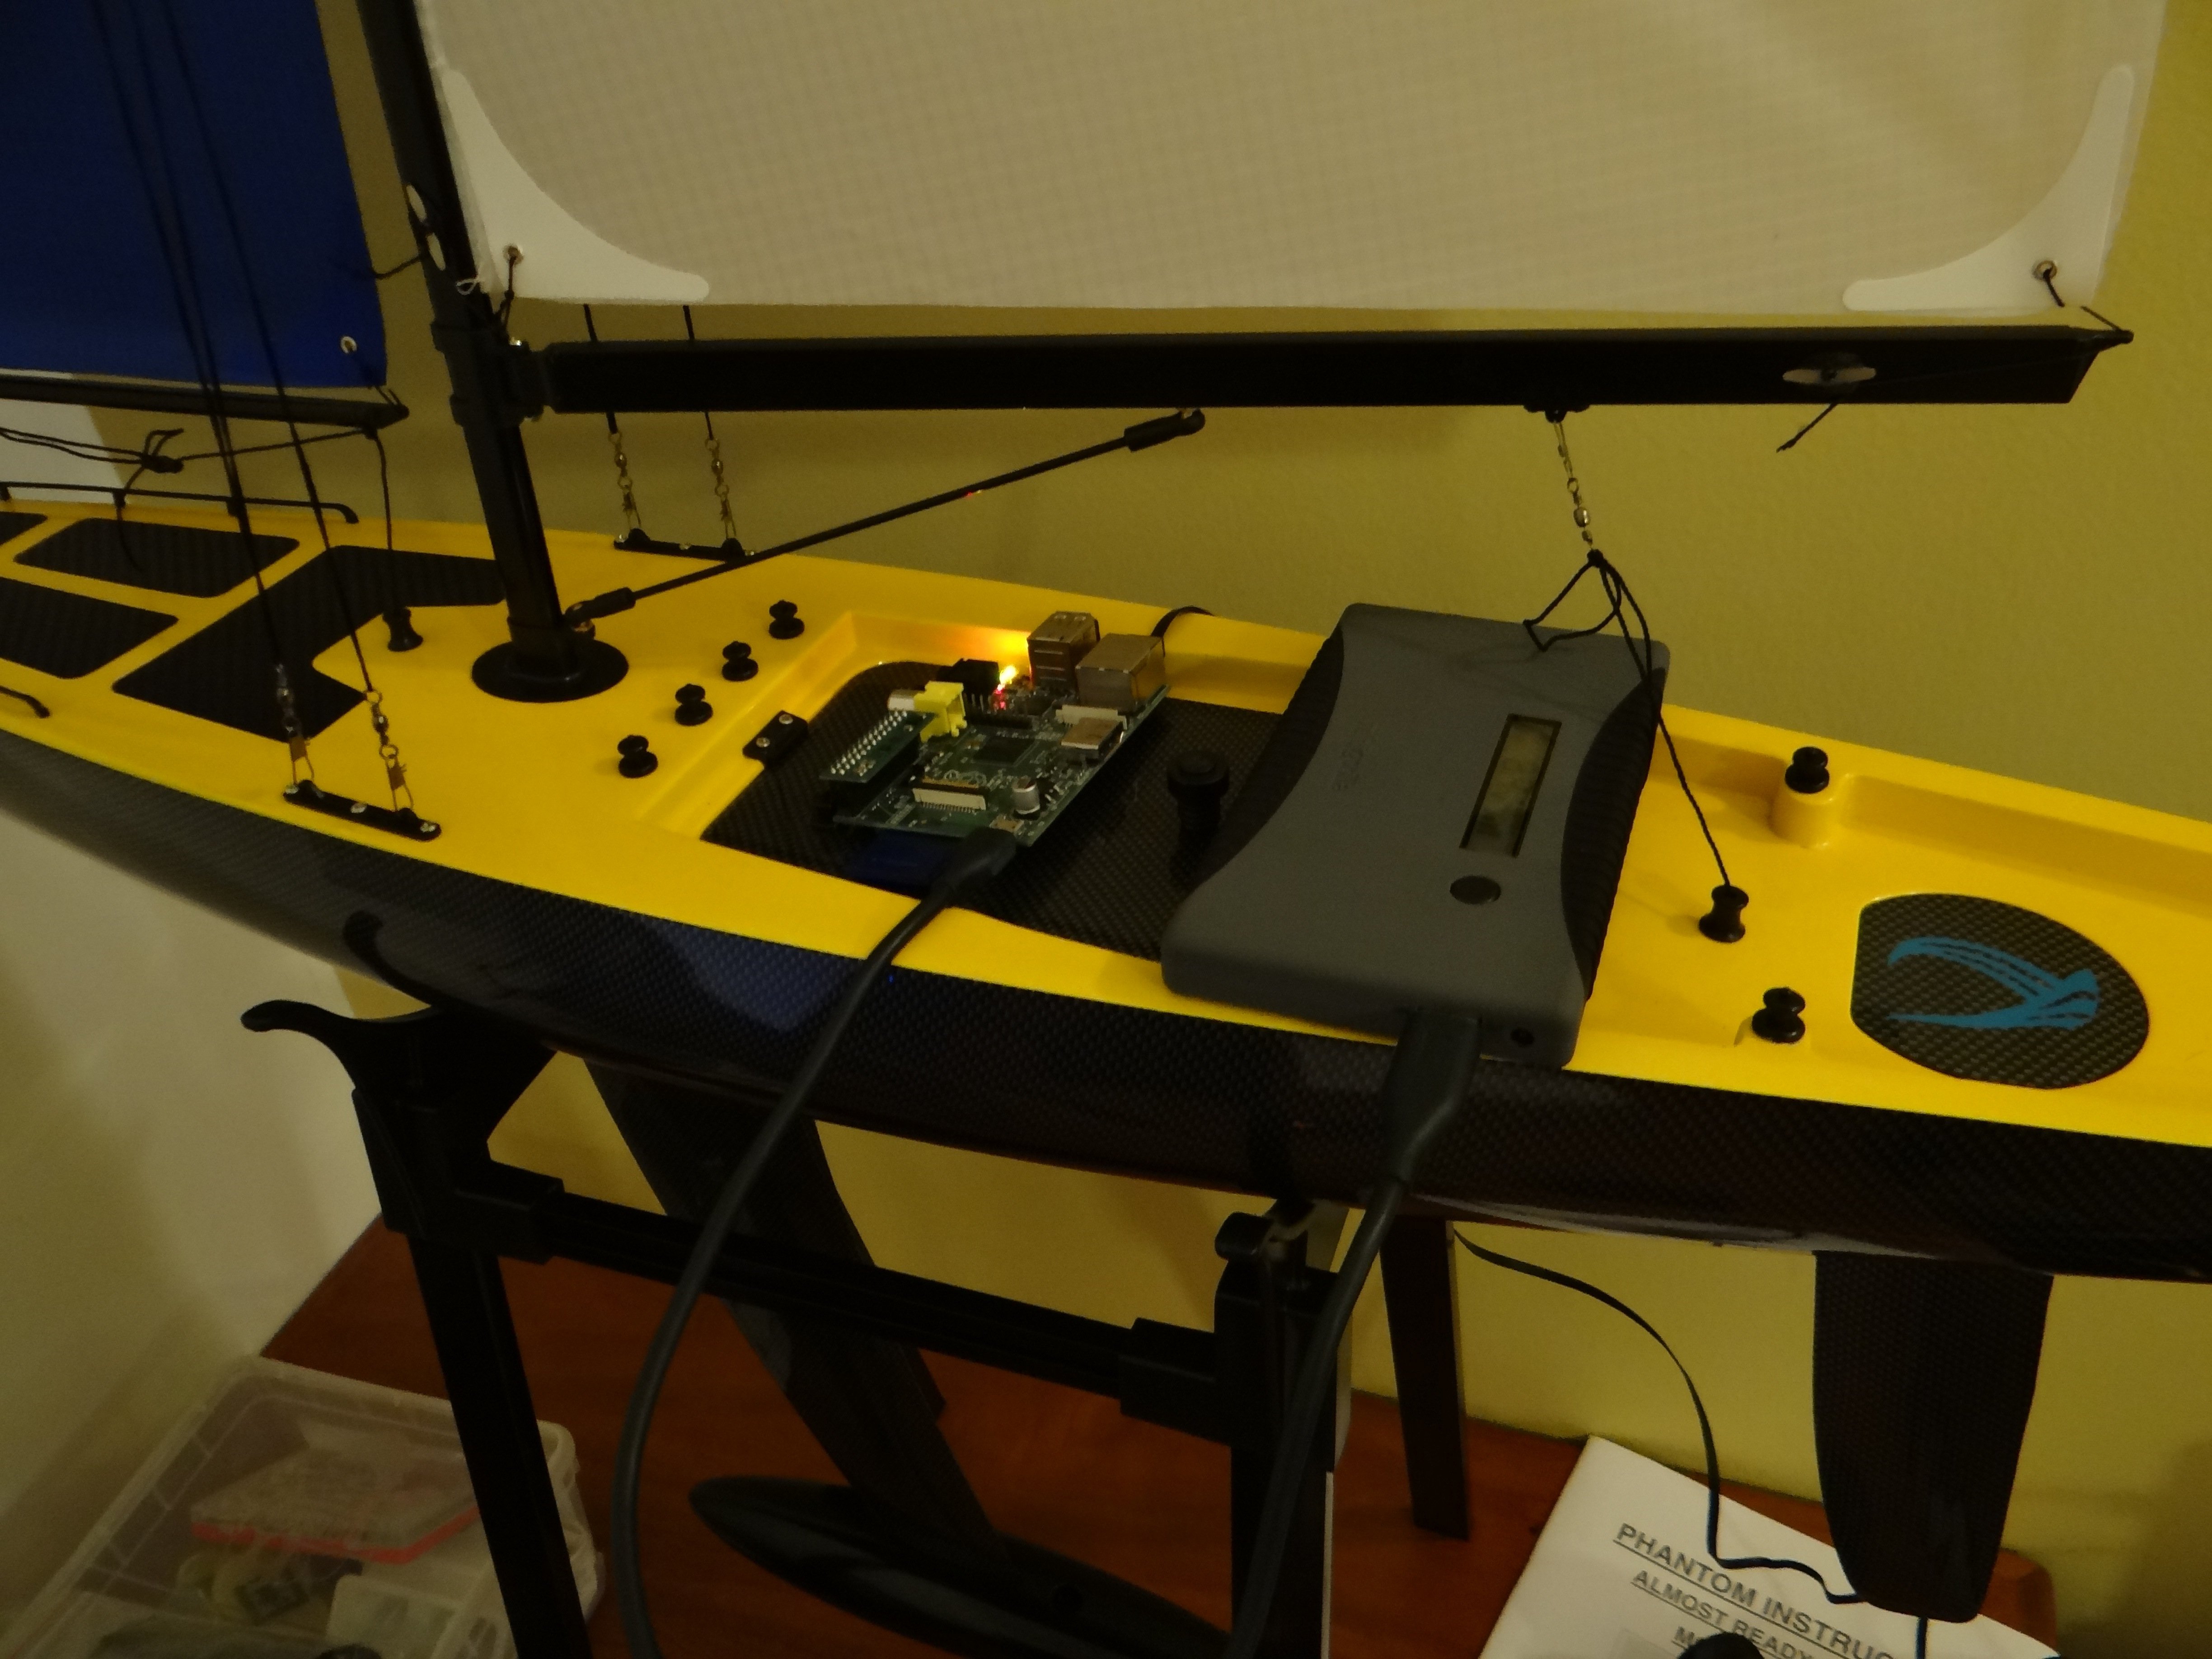
\includegraphics[width=5cm]{sailbot000}
\end{center}
\column[t]{0.5\textwidth}
\begin{center}
 Boat itself\newline\linebreak
 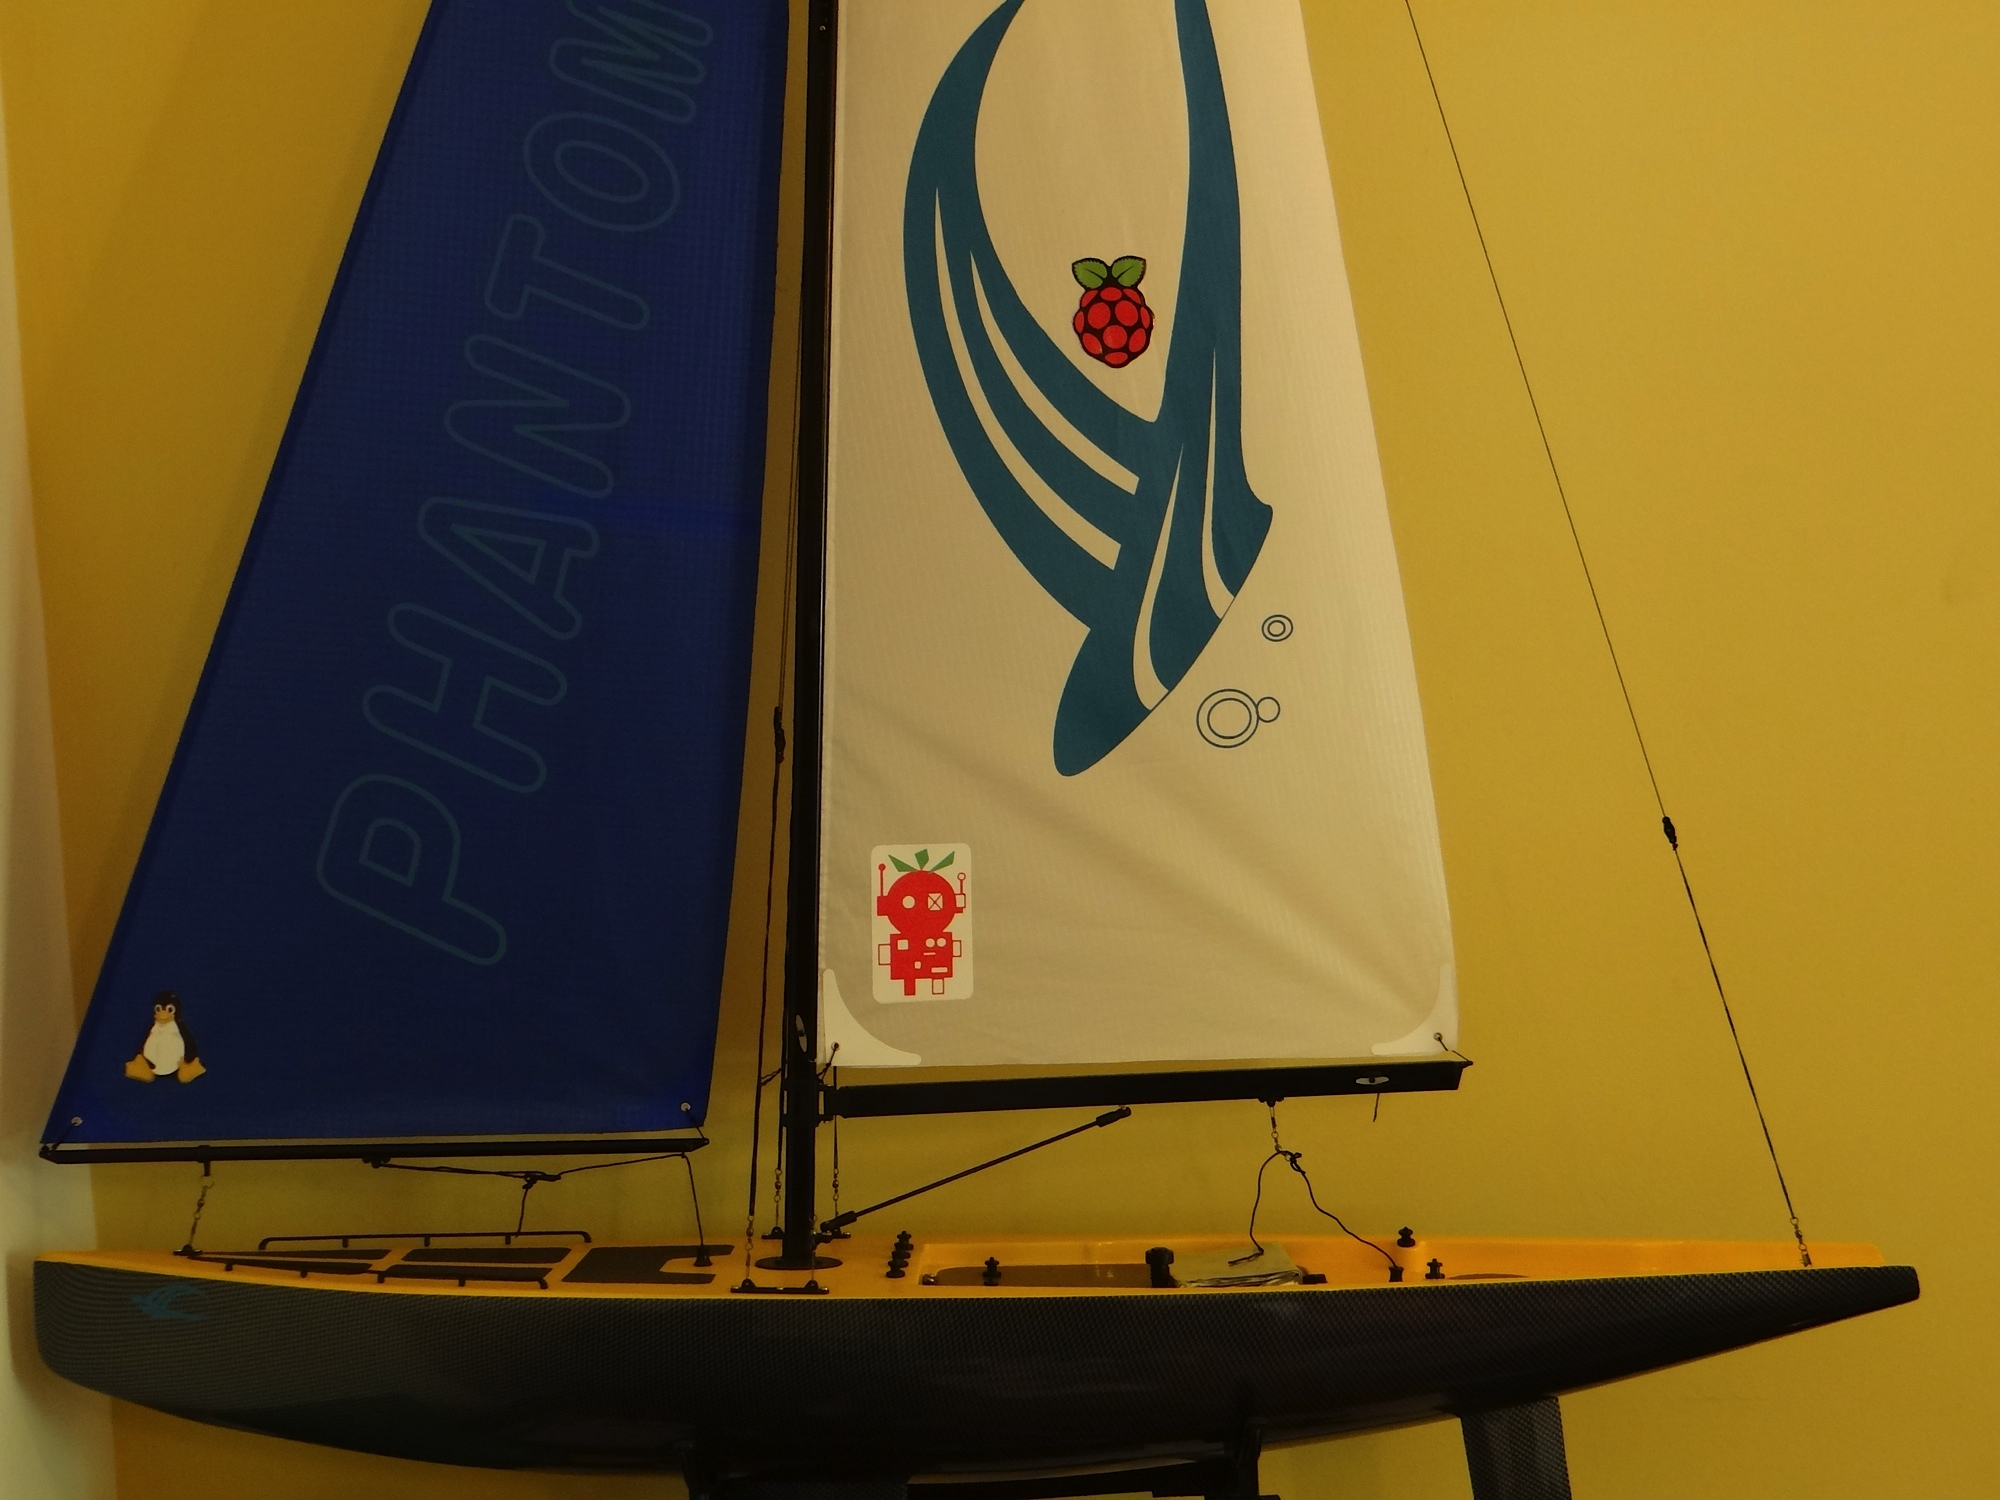
\includegraphics[width=5cm]{sailbot001}
\end{center}

\end{columns}

\end{frame}

\subsection{RaspberryPI}
%%%%%%%%%%%%%%%%%%%%%%%%%%%%%%%%%%%%%%%%%%%%%%%%%%%%%%%%%%%%%%%%%%%%
\begin{frame}[fragile]{RaspberryPI}

AmiTomi's brain is the RaspberyPI python code:

\begin{itemize}
 \item Skipper: the captain/navigator software
 \item Waypoint sorter: optimizer for route
 \item Sensor datalogger: simultaneous sensing
 \item Mapper: import data and 3D interpolation 
\end{itemize}


\begin{columns}[l]
\column[t]{0.5\textwidth}
\begin{center}
 RaspberryPI GPIO connecting to temperature sensor \newline\linebreak
 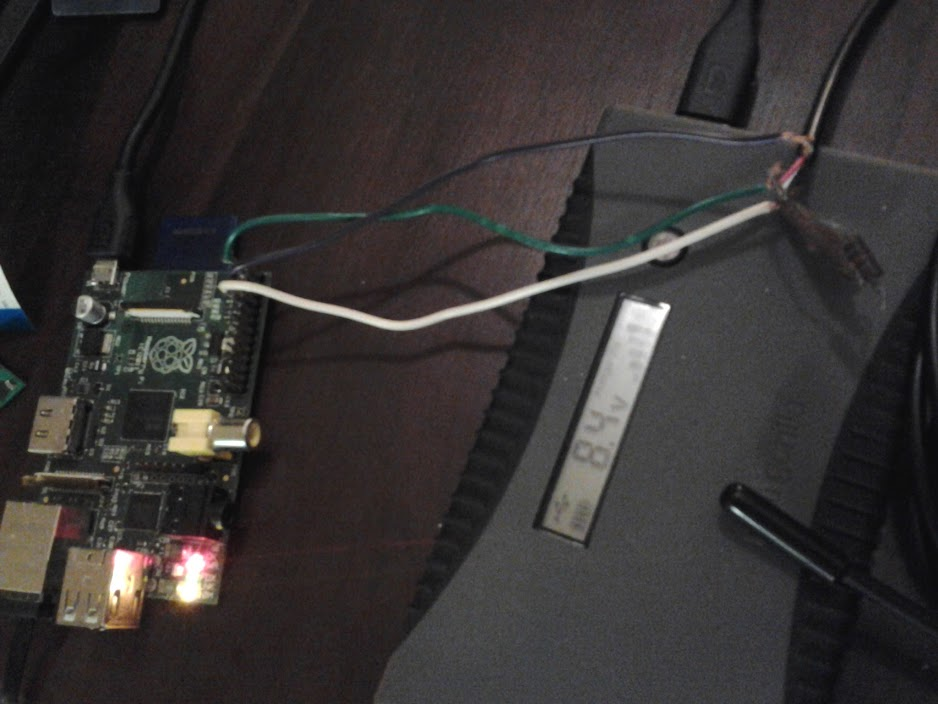
\includegraphics[width=5cm]{temperature_probe_GPIO}
\end{center}
\column[t]{0.5\textwidth}
\begin{center}
 Temperature digital sensors (2m cables)\newline\linebreak
 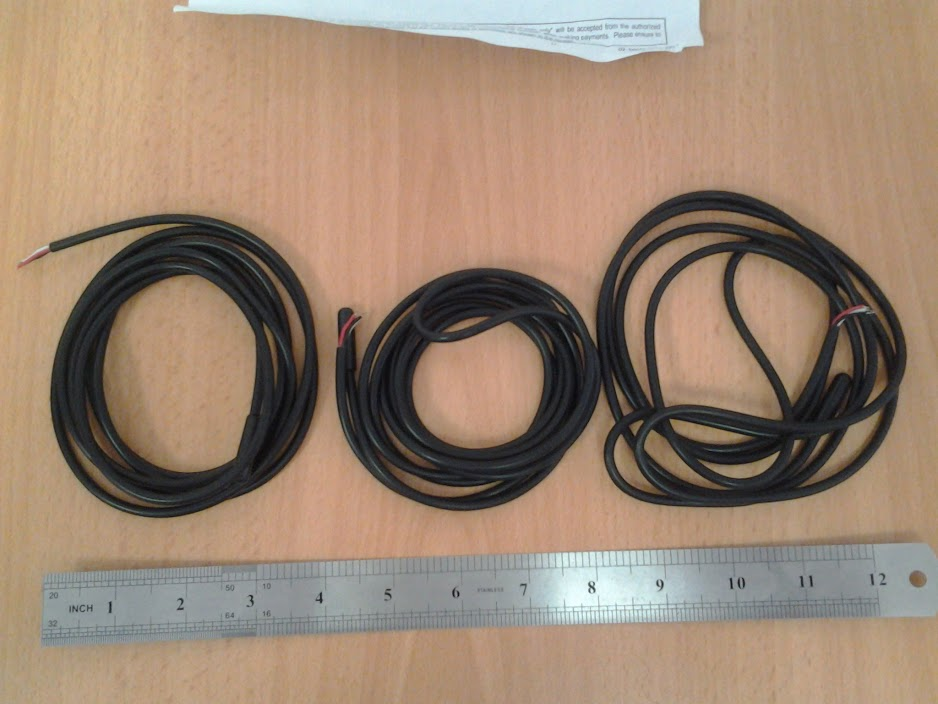
\includegraphics[width=5cm]{temperature_probe_waterproof}
\end{center}
\end{columns}

\end{frame}

\subsection{Sensors}
%%%%%%%%%%%%%%%%%%%%%%%%%%%%%%%%%%%%%%%%%%%%%%%%%%%%%%%%%%%%%%%%%%%%
\begin{frame}[fragile]{Evaporation Monitoring Experiment}

\begin{center}
 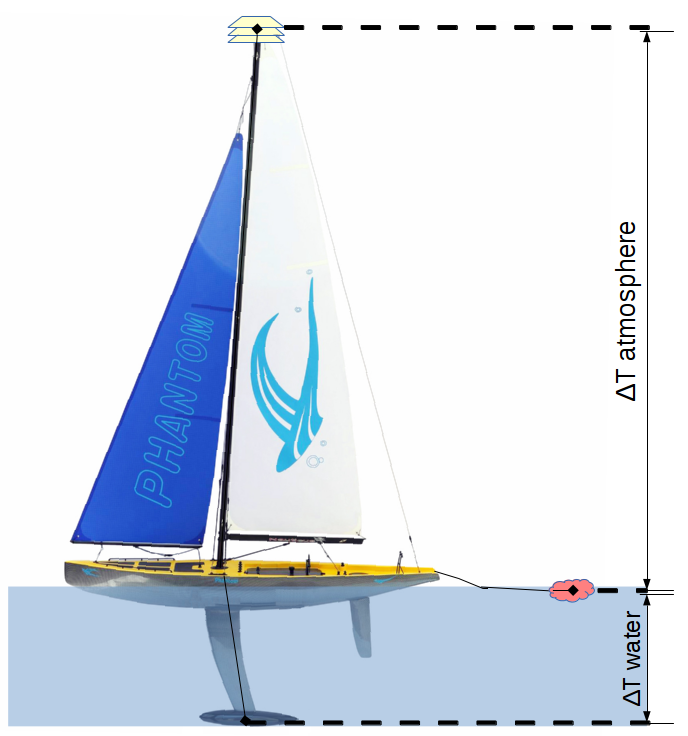
\includegraphics[width=8cm]{amitomiv1}
\end{center}

\end{frame}


\subsection{FOSS4G}
%%%%%%%%%%%%%%%%%%%%%%%%%%%%%%%%%%%%%%%%%%%%%%%%%%%%%%%%%%%%%%%%%%%%
\begin{frame}[fragile]{FOSS4G software}

\begin{itemize}
 \item Python-gps (GPS data)
 \item Python-i2ctools (Compass/Temperature data)
 \item Python-XloBorg (Compass data)
 \item Python-openopt (Waypoints downwind sorting \href{htp://openopt.org}{openopt.org})
 \item Python-MotorPiTX (servo control for sails \& rudder)
 \item (py)GRASS (live processing of 3D GIS data)
 \item If online: PyWPS, SOS/network reporting. 
\end{itemize}

\end{frame}

\section{Conclusions}
%%%%%%%%%%%%%%%%%%%%%%%%%%%%%%%%%%%%%%%%%%%%%%%%%%%%%%%%%%%%%%%%%%%%
\begin{frame}[fragile]{Conclusions}

\begin{block}{FOSS4G natural extension is Open Source Hardware}
\begin{itemize}
 \item {\bf RaspberryPI:} Small PC (ARM v8, Linux) 
 \item {\bf Arduino:} Micro-controller
 \item {\bf OpenLog:} Data Logger
 \item {\bf GDAL/OGR:} Flexible sensor raw data manipulation
 \item {\bf GRASS GIS:} Mobile FOSS4G powerhouse
 \item {\bf PyWPS:} Online GRASS GIS processing 
 \item {\bf Together:} Flexible all-in-one sensor-to-map solutions
\end{itemize}
\end{block}

\end{frame}

%%%%%%%%%%%%%%%%%%%%%%%%%%%%%%%%%%%%%%%%%%%%%%%%%%%%%%%%%%%%%%%%%%%%
\begin{frame}[fragile]{Thank You}

\begin{center}
 
\includegraphics[height=6cm]{ohm}
\end{center}

\begin{flushright}
 
\includegraphics[height=0.9cm]{iwmi}
 \hspace{5mm}
 
\includegraphics[height=1cm]{uoMoratuwa}
 \hspace{5mm}
 
\includegraphics[height=1cm]{uoMoratuwa_foa}
\end{flushright}

\end{frame}

\end{document}
